\section{Математическое описание}

\subsection{Булева функция и её таблица истинности.}

Функции $f: E_2^n \to E_2$, где $E_2 = \{0, 1\}$, называются функциями алгебры логики, или булевыми функциями от $n$ переменных, по имени Дж.~Буля.

В данной работе рассматривается функция $f(x_1, x_2, x_3, x_4)$ четырёх переменных, заданная вектором значений. Функция задана десятичным числом 11011, которое в двоичной системе счисления (с заполнением первых разрядом нулями, пока не достигнем 16 разрядов) имеет вид:
\[
11011_{10} = 0010101100000011_2.
\]

Таблица истинности~--- это способ задания булевой функции, в котором для каждого из $2^n$ наборов значений переменных указано значение функции. Таблица истинности для заданной булевой функции представлена в таблице~\ref{tab:truth-table}.

\begin{table}[H]
\centering
\begin{tabular}{|c|c|c|c|c|c|}
\hline
№ & $x_1$ & $x_2$ & $x_3$ & $x_4$ & $f$ \\
\hline
0  & 0 & 0 & 0 & 0 & 0 \\
1  & 0 & 0 & 0 & 1 & 0 \\
2  & 0 & 0 & 1 & 0 & 1 \\
3  & 0 & 0 & 1 & 1 & 0 \\
4  & 0 & 1 & 0 & 0 & 1 \\
5  & 0 & 1 & 0 & 1 & 0 \\
6  & 0 & 1 & 1 & 0 & 1 \\
7  & 0 & 1 & 1 & 1 & 1 \\
8  & 1 & 0 & 0 & 0 & 0 \\
9  & 1 & 0 & 0 & 1 & 0 \\
10 & 1 & 0 & 1 & 0 & 0 \\
11 & 1 & 0 & 1 & 1 & 0 \\
12 & 1 & 1 & 0 & 0 & 0 \\
13 & 1 & 1 & 0 & 1 & 0 \\
14 & 1 & 1 & 1 & 0 & 1 \\
15 & 1 & 1 & 1 & 1 & 1 \\
\hline
\end{tabular}
\caption{Таблица истинности функции $f(x_1, x_2, x_3, x_4)$}
\label{tab:truth-table}
\end{table}

\subsection{Совершенная дизъюнктивная нормальная форма.}

Булева функция $f(x_1, \ldots, x_n)$ представима в виде формулы:
\[
\bigvee_{\{(\sigma_1,\ldots,\sigma_n) \mid f(\sigma_1,\ldots,\sigma_n)=1\}} x_1^{\sigma_1} \land \ldots \land x_n^{\sigma_n}.
\]
Такая запись называется совершенной дизъюнктивной нормальной формой (СДНФ). Всякая булева функция имеет единственную СДНФ.

Для заданной функции:
\begin{multline*}
\text{СДНФ } f = \overline{x_1}\,\overline{x_2}\,x_3\,\overline{x_4} \lor \overline{x_1}\,x_2\,\overline{x_3}\,\overline{x_4} \lor \overline{x_1}\,x_2\,x_3\,\overline{x_4} \lor \overline{x_1}\,x_2\,x_3\,x_4 \lor {} \\
{}  \lor x_1\,x_2\,x_3\,\overline{x_4} \lor x_1\,x_2\,x_3\,x_4
\end{multline*}

\subsection{Совершенная конъюнктивная нормальная форма.}

Булева функция $f(x_1, \ldots, x_n)$ представима в виде формулы:
\[
\bigwedge_{\{(\sigma_1,\ldots,\sigma_n) \mid f(\sigma_1,\ldots,\sigma_n)=0\}} (x_1^{\overline{\sigma_1}} \lor \ldots \lor x_n^{\overline{\sigma_n}}).
\]
Такая запись называется совершенной конъюнктивной нормальной формой (СКНФ). Всякая булева функция имеет единственную СКНФ.

Для заданной функции (f=0 на наборах 0, 1, 3, 5, 8, 9, 10, 11, 12, 13):
\begin{multline*}
\text{СКНФ } f = (x_1 \lor x_2 \lor x_3 \lor x_4) \land (x_1 \lor x_2 \lor x_3 \lor \overline{x_4}) \land (x_1 \lor x_2 \lor \overline{x_3} \lor \overline{x_4}) \land {} \\
{} \land (x_1 \lor \overline{x_2} \lor x_3 \lor \overline{x_4}) \land (\overline{x_1} \lor x_2 \lor x_3 \lor x_4) \land (\overline{x_1} \lor x_2 \lor x_3 \lor \overline{x_4}) \land {} \\
{} \land (\overline{x_1} \lor x_2 \lor \overline{x_3} \lor x_4) \land (\overline{x_1} \lor x_2 \lor \overline{x_3} \lor \overline{x_4}) \land (\overline{x_1} \lor \overline{x_2} \lor x_3 \lor x_4) \land {} \\
{} \land (\overline{x_1} \lor \overline{x_2} \lor x_3 \lor \overline{x_4})
\end{multline*}

\subsection{Полином Жегалкина.}

Полином Жегалкина~--- представление булевой функции в базисе $\{\land, \oplus, 1\}$, где $\oplus$~--- сложение по модулю 2.

Полином Жегалкина имеет вид:
\[
f(x_1, \ldots, x_n) = a_0 \oplus \bigoplus_{i} a_i x_i \oplus \bigoplus_{i<j} a_{ij} x_i x_j \oplus \ldots \oplus a_{12\ldots n} x_1 x_2 \ldots x_n.
\]

Для заданной функции полином Жегалкина, вычисленный методом треугольника:
\[
f = x_3 \oplus x_3 x_4 \oplus x_2 \oplus x_2 x_4 \oplus x_2 x_3 \oplus x_1 x_3 \oplus x_1 x_3 x_4 \oplus x_1 x_2 \oplus x_1 x_2 x_4.
\]

\subsection{Выбор порядка переменных.} 

Порядок следования переменных выбирается с целью получения наиболее компактной бинарной диаграммы решений.

Производная показывает, на каких наборах значение функции меняется при изменении $x_i$. Чем больше единиц в таблице истинности производной, тем сильнее функция зависит от переменной.

Количество единиц в таблице истинности производных (см. раздел <<производные булевой функции>>):
\begin{itemize}
    \item $\dfrac{\partial f}{\partial x_1}$: 2 единицы~--- функция слабо зависит от $x_1$
    \item $\dfrac{\partial f}{\partial x_2}$: 4 единицы~--- функция сильно зависит от $x_2$
    \item $\dfrac{\partial f}{\partial x_3}$: 4 единицы~--- функция сильно зависит от $x_3$
    \item $\dfrac{\partial f}{\partial x_4}$: 2 единицы~--- функция слабо зависит от $x_4$
\end{itemize}

Для построения компактной БДР важно не только количество единиц в производных, но и возможность объединения эквивалентных поддеревьев. Проанализируем поведение функции при фиксации переменных.

Для упрощения оценки рассмотрим ДНФ, мининизированную с помощью алгеброических преобразований: 

\begin{align*}
f &= \overline{x_1}\,\overline{x_2}\,x_3\,\overline{x_4} \lor \overline{x_1}\,x_2\,\overline{x_3}\,\overline{x_4} \lor \overline{x_1}\,x_2\,x_3\,\overline{x_4} \lor \overline{x_1}\,x_2\,x_3\,x_4 \lor x_1\,x_2\,x_3\,\overline{x_4} \lor x_1\,x_2\,x_3\,x_4 \\
&= \overline{x_1}\,\overline{x_2}\,x_3\,\overline{x_4} \lor \overline{x_1}\,x_2\,\overline{x_3}\,\overline{x_4} \lor \overline{x_1}\,x_2\,x_3 \lor x_1\,x_2\,x_3 \\
&= \overline{x_1}\,\overline{x_2}\,x_3\,\overline{x_4} \lor \overline{x_1}\,x_2\,\overline{x_3}\,\overline{x_4} \lor x_2\,x_3 \\
\end{align*}

\begin{itemize}
    \item При $x_1 = 1$: первые два терма обнуляются, и функция упрощается до $f = x_2\,x_3$. Это означает, что при $x_1 = 1$ всё поддерево заменяется простой функцией двух переменных.
    
    \item При $x_1 = 1$ значение функции не зависит от $x_4$, что позволяет пропустить проверку $x_4$ в этой ветви.
    
    \item При $x_1 = 0$ и $x_4 = 1$: функция также упрощается до $f = x_2\,x_3$. Поддеревья при $(x_1 = 1)$ и $(x_1 = 0, x_4 = 1)$ эквивалентны и могут быть объединены в БДР.
\end{itemize}

Таким образом, если поставить $x_1$ первой переменной, а $x_4$ второй, то:
\begin{itemize}
    \item при $x_1 = 1$ можно полностью исключить проверку $x_4$;
    \item поддеревья для $(x_1 = 1)$ и $(x_1 = 0, x_4 = 1)$ совпадают и объединяются.
\end{itemize}

Выбираем порядок переменных: $x_1, x_4, x_2, x_3$.

\subsection{Семантическое дерево.} 

Таблицу истинности булевой функции $n$ переменных можно представить в виде бинарного дерева высоты $n+1$. Ярусы дерева соответствуют переменным, дуги~--- значениям переменных (пунктирная линия~--- 0, сплошная~--- 1).

Семантическое дерево для заданной функции с порядком переменных $x_1, x_4, x_2, x_3$ представлено на рис.~\ref{fig:semantic-tree}.

\begin{figure}[H]
\centering
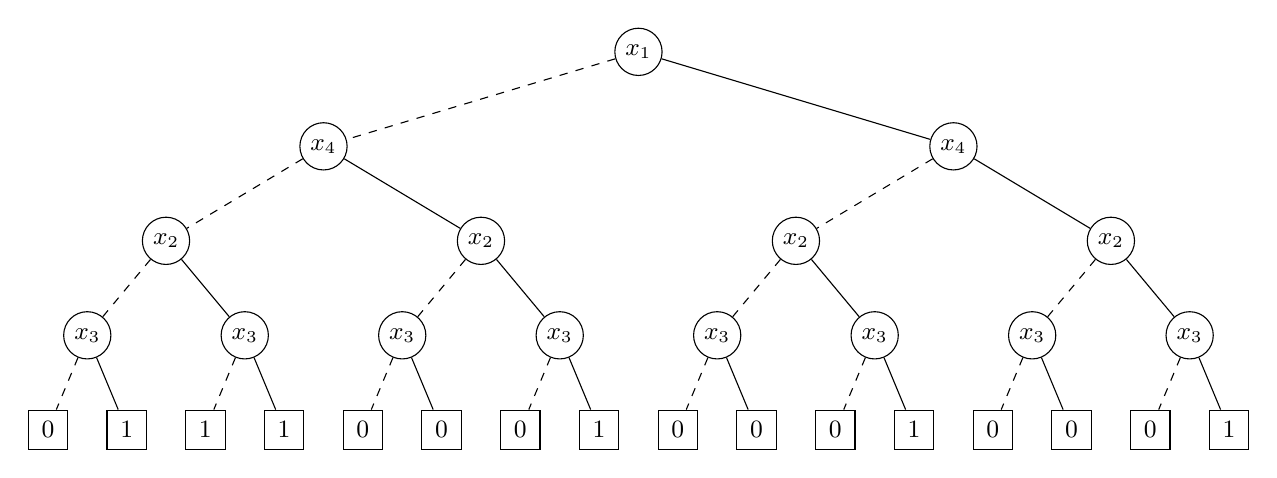
\begin{tikzpicture}[
    level 1/.style={sibling distance=80mm, level distance=12mm},
    level 2/.style={sibling distance=40mm, level distance=12mm},
    level 3/.style={sibling distance=20mm, level distance=12mm},
    level 4/.style={sibling distance=10mm, level distance=12mm},
    every node/.style={circle, draw, solid, minimum size=6mm, inner sep=1pt, font=\small},
    leaf/.style={rectangle, draw, solid, minimum size=5mm, inner sep=2pt, font=\small},
    edge0/.style={dashed},
    edge1/.style={solid}
]
\node {$x_1$}
    child {node {$x_4$}
        child {node {$x_2$}
            child {node {$x_3$}
                child {node[leaf] {0} edge from parent[edge0]}
                child {node[leaf] {1} edge from parent[edge1]}
                edge from parent[edge0]
            }
            child {node {$x_3$}
                child {node[leaf] {1} edge from parent[edge0]}
                child {node[leaf] {1} edge from parent[edge1]}
                edge from parent[edge1]
            }
            edge from parent[edge0]
        }
        child {node {$x_2$}
            child {node {$x_3$}
                child {node[leaf] {0} edge from parent[edge0]}
                child {node[leaf] {0} edge from parent[edge1]}
                edge from parent[edge0]
            }
            child {node {$x_3$}
                child {node[leaf] {0} edge from parent[edge0]}
                child {node[leaf] {1} edge from parent[edge1]}
                edge from parent[edge1]
            }
            edge from parent[edge1]
        }
        edge from parent[edge0]
    }
    child {node {$x_4$}
        child {node {$x_2$}
            child {node {$x_3$}
                child {node[leaf] {0} edge from parent[edge0]}
                child {node[leaf] {0} edge from parent[edge1]}
                edge from parent[edge0]
            }
            child {node {$x_3$}
                child {node[leaf] {0} edge from parent[edge0]}
                child {node[leaf] {1} edge from parent[edge1]}
                edge from parent[edge1]
            }
            edge from parent[edge0]
        }
        child {node {$x_2$}
            child {node {$x_3$}
                child {node[leaf] {0} edge from parent[edge0]}
                child {node[leaf] {0} edge from parent[edge1]}
                edge from parent[edge0]
            }
            child {node {$x_3$}
                child {node[leaf] {0} edge from parent[edge0]}
                child {node[leaf] {1} edge from parent[edge1]}
                edge from parent[edge1]
            }
            edge from parent[edge1]
        }
        edge from parent[edge1]
    };
\end{tikzpicture}
\caption{Семантическое дерево функции $f$ (порядок $x_1, x_4, x_2, x_3$)}
\label{fig:semantic-tree}
\end{figure}

\subsection{Упрощённое семантическое дерево.}

Упрощённое семантическое дерево представлено на рис.~\ref{fig:simplified-tree}. При упрощении применяются следующие правила:
\begin{itemize}
    \item если оба потомка узла~--- одинаковые листья, узел заменяется этим листом;
    \item если поддеревья эквивалентны, они объединяются.
\end{itemize}

\begin{figure}[H]
\centering
\begin{tikzpicture}[
    level 1/.style={sibling distance=60mm, level distance=15mm},
    level 2/.style={sibling distance=35mm, level distance=15mm},
    level 3/.style={sibling distance=18mm, level distance=15mm},
    node/.style={circle, draw, solid, minimum size=8mm, inner sep=1pt, font=\small},
    leaf/.style={rectangle, draw, solid, minimum size=7mm, inner sep=2pt, font=\small},
    edge0/.style={dashed},
    edge1/.style={solid}
]
\node[node] {$x_1$}
    child {node[node] {$x_4$}
        child {node[node] {$x_2$}
            child {node[node] {$x_3$}
                child {node[leaf] {0} edge from parent[edge0]}
                child {node[leaf] {1} edge from parent[edge1]}
                edge from parent[edge0]
            }
            child {node[leaf] {1} edge from parent[edge1]}
            edge from parent[edge0]
        }
        child {node[node] {$x_2$}
            child {node[leaf] {0} edge from parent[edge0]}
            child {node[node] {$x_3$}
                child {node[leaf] {0} edge from parent[edge0]}
                child {node[leaf] {1} edge from parent[edge1]}
                edge from parent[edge1]
            }
            edge from parent[edge1]
        }
        edge from parent[edge0]
    }
    child {node[node] {$x_2$}
        child {node[leaf] {0} edge from parent[edge0]}
        child {node[node] {$x_3$}
            child {node[leaf] {0} edge from parent[edge0]}
            child {node[leaf] {1} edge from parent[edge1]}
            edge from parent[edge1]
        }
        edge from parent[edge1]
    };
\end{tikzpicture}
\caption{Упрощённое семантическое дерево функции $f$ (порядок $x_1, x_4, x_2, x_3$)}
\label{fig:simplified-tree}
\end{figure}

При упрощении:
\begin{itemize}
    \item При $x_1 = 1$ проверка $x_4$ пропускается, так как результат не зависит от $x_4$.
    \item Поддерево при $x_1 = 1$ совпадает с поддеревом при $(x_1 = 0, x_4 = 1)$.
    \item Узлы $x_3$ с одинаковыми потомками $(0, 1)$ объединяются.
\end{itemize}

\subsection{Бинарная диаграмма решений.}

Бинарная диаграмма решений (БДР) для заданной функции представлена на рис.~\ref{fig:bdd-graph}. В БДР, в отличие от дерева, допускается повторное использование узлов~--- эквивалентные поддеревья представляются одним подграфом.

\begin{figure}[H]
\centering
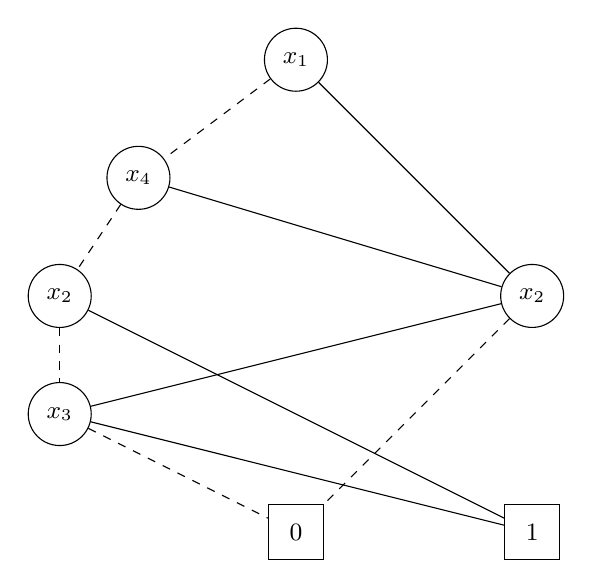
\begin{tikzpicture}[
    node/.style={circle, draw, solid, minimum size=8mm, inner sep=1pt, font=\small},
    leaf/.style={rectangle, draw, solid, minimum size=7mm, inner sep=2pt, font=\small},
    edge0/.style={dashed},
    edge1/.style={solid}
]
% Уровень 1
\node[node] (x1) at (0, 0) {$x_1$};

% Уровень 2
\node[node] (x4) at (-2, -1.5) {$x_4$};
\node[node] (x2b) at (3, -3) {$x_2$};

% Уровень 3
\node[node] (x2a) at (-3, -3) {$x_2$};

% Уровень 4
\node[node] (x3b) at (-3, -4.5) {$x_3$};

% Листья
\node[leaf] (l0) at (0, -6) {0};
\node[leaf] (l1) at (3, -6) {1};

% Рёбра от x1
\draw[edge0] (x1) -- (x4);
\draw[edge1] (x1) -- (x2b);

% Рёбра от x4
\draw[edge0] (x4) -- (x2a);
\draw[edge1] (x4) -- (x2b);

% Рёбра от x2a
\draw[edge0] (x2a) -- (x3b);
\draw[edge1] (x2a) -- (l1);

% Рёбра от x2b
\draw[edge1] (x2b) -- (x3b);
\draw[edge0] (x2b) -- (l0);

% Рёбра от x3b
\draw[edge0] (x3b) -- (l0);
\draw[edge1] (x3b) -- (l1);
\end{tikzpicture}
\caption{Бинарная диаграмма решений (пунктир~--- 0, сплошная~--- 1)}
\label{fig:bdd-graph}
\end{figure}

ДНФ из БДР: $f = \overline{x_1}\,\overline{x_2}\,x_3\,\overline{x_4} \lor \overline{x_1}\,x_2\,\overline{x_4} \lor \overline{x_1}\,x_2\,x_3\,x_4 \lor x_1\,x_2\,x_3$.

После упрощения даёт: $f = \overline{x_1}\,x_3\,\overline{x_4} \lor \overline{x_1}\,x_2\,\overline{x_4} \lor x_2\,x_3$.

\begin{itemize}
    \item Терм $\overline{x_1}\,\overline{x_2}\,x_3\,\overline{x_4} \lor \overline{x_1}\,x_2\,x_3\,x_4 = \overline{x_1}\,x_3\,\overline{x_4}$ (поглощение по $x_2$).
    \item Термы $\overline{x_1}\,x_2\,x_3\,x_4$ и $x_1\,x_2\,x_3$ объединяются: $x_2\,x_3\,(\overline{x_1}\,x_4 \lor x_1) = x_2\,x_3\,(x_1 \lor x_4)$, что после упрощения даёт $x_2\,x_3$.
\end{itemize}

Таким образом, БДР даёт сокращённую форму, которую в дальнейшем можно использовать для построения логической схемы.

\subsection{Синтаксическое дерево минимальной ДНФ.} 

Синтаксическое дерево~--- это представление формулы в виде дерева, где внутренние вершины соответствуют операциям, а листья~--- переменным или константам.

Синтаксическое дерево для минимальной ДНФ $f = \overline{x_1}\,x_3\,\overline{x_4} \lor \overline{x_1}\,x_2\,\overline{x_4} \lor x_2\,x_3$ представлено на рис.~\ref{fig:syntax-tree}.

\begin{figure}[H]
\centering
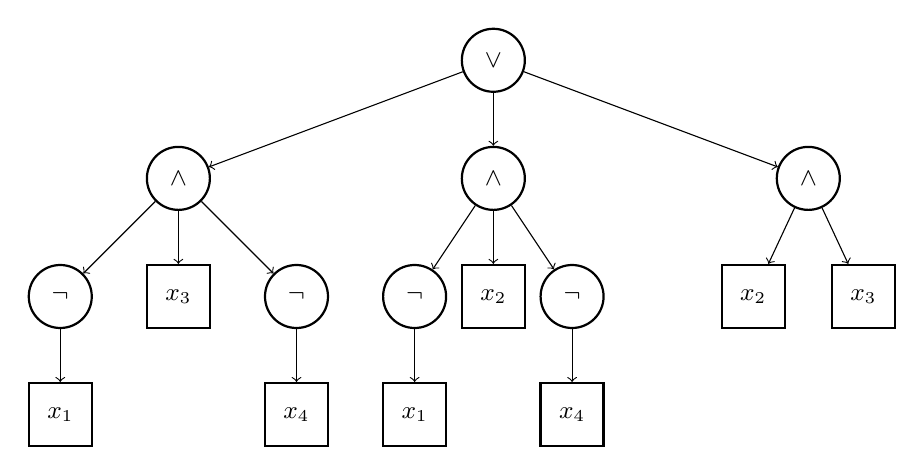
\begin{tikzpicture}[
    op/.style={circle, draw, thick, minimum size=8mm, font=\small},
    var/.style={rectangle, draw, thick, minimum size=8mm, font=\small},
]

% Уровень 0: корень
\node[op] (root) at (0, 0) {$\lor$};

% Уровень 1: три конъюнкции
\node[op] (and1) at (-4, -1.5) {$\land$};
\node[op] (and2) at (0, -1.5) {$\land$};
\node[op] (and3) at (4, -1.5) {$\land$};

% Уровень 2: операнды первой конъюнкции
\node[op] (neg1) at (-5.5, -3) {$\neg$};
\node[var] (x3a) at (-4, -3) {$x_3$};
\node[op] (neg2) at (-2.5, -3) {$\neg$};

% Уровень 2: операнды второй конъюнкции
\node[op] (neg3) at (-1, -3) {$\neg$};
\node[var] (x2a) at (0, -3) {$x_2$};
\node[op] (neg4) at (1, -3) {$\neg$};

% Уровень 2: операнды третьей конъюнкции
\node[var] (x2b) at (3.3, -3) {$x_2$};
\node[var] (x3b) at (4.7, -3) {$x_3$};

% Уровень 3: переменные под отрицаниями
\node[var] (x1a) at (-5.5, -4.5) {$x_1$};
\node[var] (x4a) at (-2.5, -4.5) {$x_4$};
\node[var] (x1b) at (-1, -4.5) {$x_1$};
\node[var] (x4b) at (1, -4.5) {$x_4$};

% Рёбра от корня
\draw[->] (root) -- (and1);
\draw[->] (root) -- (and2);
\draw[->] (root) -- (and3);

% Рёбра первой конъюнкции
\draw[->] (and1) -- (neg1);
\draw[->] (and1) -- (x3a);
\draw[->] (and1) -- (neg2);

% Рёбра второй конъюнкции
\draw[->] (and2) -- (neg3);
\draw[->] (and2) -- (x2a);
\draw[->] (and2) -- (neg4);

% Рёбра третьей конъюнкции
\draw[->] (and3) -- (x2b);
\draw[->] (and3) -- (x3b);

% Рёбра отрицаний
\draw[->] (neg1) -- (x1a);
\draw[->] (neg2) -- (x4a);
\draw[->] (neg3) -- (x1b);
\draw[->] (neg4) -- (x4b);

\end{tikzpicture}
\caption{Синтаксическое дерево минимальной ДНФ}
\label{fig:syntax-tree}
\end{figure}

\subsection{Логическая схема.}

Логическая схема~--- это схема, реализующая булеву функцию с помощью логических элементов (И, ИЛИ, НЕ).

\screenshot{image_2026-01-15_05-18-09.png}{Логическая схема для минимальной ДНФ}

\subsection{Производные булевой функции.} 

Производная булевой функции $f$ по переменной $x_i$:
\[
\frac{\partial f}{\partial x_i} = f|_{x_i = 0} \oplus f|_{x_i = 1}.
\]


Вычислим производные функции $f = \overline{x_1}\,x_3\,\overline{x_4} \lor \overline{x_1}\,x_2\,\overline{x_4} \lor x_2\,x_3$ по каждой переменной.

\subsubsection*{Производная по $x_1$.}

\[
f|_{x_1=0} = \overline{0}\,x_3\,\overline{x_4} \lor \overline{0}\,x_2\,\overline{x_4} \lor x_2\,x_3 = x_3\,\overline{x_4} \lor x_2\,\overline{x_4} \lor x_2\,x_3.
\]

\[
f|_{x_1=1} = \overline{1}\,x_3\,\overline{x_4} \lor \overline{1}\,x_2\,\overline{x_4} \lor x_2\,x_3 = 0 \lor 0 \lor x_2\,x_3 = x_2\,x_3.
\]

\begin{align*}
\frac{\partial f}{\partial x_1} &= f|_{x_1=0} \oplus f|_{x_1=1} = (x_3\,\overline{x_4} \lor x_2\,\overline{x_4} \lor x_2\,x_3) \oplus (x_2\,x_3) \\
&= (x_3\,\overline{x_4} \lor x_2\,\overline{x_4} \lor x_2\,x_3) \cdot \overline{x_2\,x_3} \lor \overline{(x_3\,\overline{x_4} \lor x_2\,\overline{x_4} \lor x_2\,x_3)} \cdot x_2\,x_3.
\end{align*}

\begin{align*}
(x_3\,\overline{x_4} \lor x_2\,\overline{x_4} \lor x_2\,x_3) \cdot (\overline{x_2} \lor \overline{x_3}) &= x_3\,\overline{x_4}\,\overline{x_2} \lor x_3\,\overline{x_4}\,\overline{x_3} \lor x_2\,\overline{x_4}\,\overline{x_2} \lor x_2\,\overline{x_4}\,\overline{x_3} \\
&\quad \lor x_2\,x_3\,\overline{x_2} \lor x_2\,x_3\,\overline{x_3} \\
&= \overline{x_2}\,x_3\,\overline{x_4} \lor x_2\,\overline{x_3}\,\overline{x_4}.
\end{align*}

\[
\overline{(x_3\,\overline{x_4} \lor x_2\,\overline{x_4} \lor x_2\,x_3)} = (\overline{x_3} \lor x_4)(\overline{x_2} \lor x_4)(\overline{x_2} \lor \overline{x_3}).
\]

\[
(\overline{x_3} \lor x_4)(\overline{x_2} \lor x_4)(\overline{x_2} \lor \overline{x_3}) \cdot x_2\,x_3 = 0,
\]
так как $x_2 \cdot \overline{x_2} = 0$ и $x_3 \cdot \overline{x_3} = 0$.

Итого:
\[
\frac{\partial f}{\partial x_1} = \overline{x_2}\,x_3\,\overline{x_4} \lor x_2\,\overline{x_3}\,\overline{x_4}.
\]

\subsubsection*{Производная по $x_2$.}

\[
f|_{x_2=0} = \overline{x_1}\,x_3\,\overline{x_4} \lor \overline{x_1}\,0\,\overline{x_4} \lor 0\,x_3 = \overline{x_1}\,x_3\,\overline{x_4}.
\]

\[
f|_{x_2=1} = \overline{x_1}\,x_3\,\overline{x_4} \lor \overline{x_1}\,\overline{x_4} \lor x_3 = \overline{x_1}\,\overline{x_4} \lor x_3.
\]

\begin{align*}
\frac{\partial f}{\partial x_2} &= (\overline{x_1}\,x_3\,\overline{x_4}) \oplus (\overline{x_1}\,\overline{x_4} \lor x_3) \\
&= \overline{x_1}\,x_3\,\overline{x_4} \cdot \overline{(\overline{x_1}\,\overline{x_4} \lor x_3)} \lor \overline{\overline{x_1}\,x_3\,\overline{x_4}} \cdot (\overline{x_1}\,\overline{x_4} \lor x_3) \\
&= \overline{x_1}\,x_3\,\overline{x_4} \cdot (x_1 \lor x_4) \cdot \overline{x_3} \lor (x_1 \lor \overline{x_3} \lor x_4)(\overline{x_1}\,\overline{x_4} \lor x_3) \\
&= 0 \lor \overline{x_1}\,\overline{x_3}\,\overline{x_4} \lor x_1\,x_3 \lor x_3\,x_4 \\
&= \overline{x_1}\,\overline{x_3}\,\overline{x_4} \lor x_1\,x_3 \lor x_3\,x_4.
\end{align*}

\subsubsection*{Производная по $x_3$.}

\[
f|_{x_3=0} = \overline{x_1}\,0\,\overline{x_4} \lor \overline{x_1}\,x_2\,\overline{x_4} \lor x_2\,0 = \overline{x_1}\,x_2\,\overline{x_4}.
\]

\[
f|_{x_3=1} = \overline{x_1}\,\overline{x_4} \lor \overline{x_1}\,x_2\,\overline{x_4} \lor x_2 = \overline{x_1}\,\overline{x_4} \lor x_2.
\]

\begin{align*}
\frac{\partial f}{\partial x_3} &= (\overline{x_1}\,x_2\,\overline{x_4}) \oplus (\overline{x_1}\,\overline{x_4} \lor x_2) \\
&= \overline{x_1}\,x_2\,\overline{x_4} \cdot \overline{(\overline{x_1}\,\overline{x_4} \lor x_2)} \lor \overline{\overline{x_1}\,x_2\,\overline{x_4}} \cdot (\overline{x_1}\,\overline{x_4} \lor x_2) \\
&= 0 \lor (x_1 \lor \overline{x_2} \lor x_4)(\overline{x_1}\,\overline{x_4} \lor x_2) \\
&= \overline{x_1}\,\overline{x_2}\,\overline{x_4} \lor x_1\,x_2 \lor x_2\,x_4.
\end{align*}

\subsubsection*{Производная по $x_4$.}

\[
f|_{x_4=0} = \overline{x_1}\,x_3\,\overline{0} \lor \overline{x_1}\,x_2\,\overline{0} \lor x_2\,x_3 = \overline{x_1}\,x_3 \lor \overline{x_1}\,x_2 \lor x_2\,x_3.
\]

\[
f|_{x_4=1} = \overline{x_1}\,x_3\,\overline{1} \lor \overline{x_1}\,x_2\,\overline{1} \lor x_2\,x_3 = 0 \lor 0 \lor x_2\,x_3 = x_2\,x_3.
\]

\begin{align*}
\frac{\partial f}{\partial x_4} &= (\overline{x_1}\,x_3 \lor \overline{x_1}\,x_2 \lor x_2\,x_3) \oplus (x_2\,x_3) \\
&= (\overline{x_1}\,x_3 \lor \overline{x_1}\,x_2 \lor x_2\,x_3) \cdot \overline{x_2\,x_3} \lor \overline{(\overline{x_1}\,x_3 \lor \overline{x_1}\,x_2 \lor x_2\,x_3)} \cdot x_2\,x_3 \\
&= (\overline{x_1}\,x_3 \lor \overline{x_1}\,x_2 \lor x_2\,x_3)(\overline{x_2} \lor \overline{x_3}) \lor 0 \\
&= \overline{x_1}\,\overline{x_2}\,x_3 \lor \overline{x_1}\,x_2\,\overline{x_3}.
\end{align*}

\subsubsection*{Таблицы истинности производных.}

\begin{table}[H]
\centering
\begin{tabular}{c@{\quad}c@{\quad}c@{\quad}c}
\toprule
$x_2$ & $x_3$ & $x_4$ & $\frac{\partial f}{\partial x_1}$ \\
\midrule
0 & 0 & 0 & 0 \\
0 & 0 & 1 & 0 \\
0 & 1 & 0 & 1 \\
0 & 1 & 1 & 0 \\
1 & 0 & 0 & 1 \\
1 & 0 & 1 & 0 \\
1 & 1 & 0 & 0 \\
1 & 1 & 1 & 0 \\
\bottomrule
\end{tabular}
\hfill
\begin{tabular}{c@{\quad}c@{\quad}c@{\quad}c}
\toprule
$x_1$ & $x_3$ & $x_4$ & $\frac{\partial f}{\partial x_2}$ \\
\midrule
0 & 0 & 0 & 1 \\
0 & 0 & 1 & 0 \\
0 & 1 & 0 & 0 \\
0 & 1 & 1 & 1 \\
1 & 0 & 0 & 0 \\
1 & 0 & 1 & 0 \\
1 & 1 & 0 & 1 \\
1 & 1 & 1 & 1 \\
\bottomrule
\end{tabular}
\hfill
\begin{tabular}{c@{\quad}c@{\quad}c@{\quad}c}
\toprule
$x_1$ & $x_2$ & $x_4$ & $\frac{\partial f}{\partial x_3}$ \\
\midrule
0 & 0 & 0 & 1 \\
0 & 0 & 1 & 0 \\
0 & 1 & 0 & 0 \\
0 & 1 & 1 & 1 \\
1 & 0 & 0 & 0 \\
1 & 0 & 1 & 0 \\
1 & 1 & 0 & 1 \\
1 & 1 & 1 & 1 \\
\bottomrule
\end{tabular}
\hfill
\begin{tabular}{c@{\quad}c@{\quad}c@{\quad}c}
\toprule
$x_1$ & $x_2$ & $x_3$ & $\frac{\partial f}{\partial x_4}$ \\
\midrule
0 & 0 & 0 & 0 \\
0 & 0 & 1 & 1 \\
0 & 1 & 0 & 1 \\
0 & 1 & 1 & 0 \\
1 & 0 & 0 & 0 \\
1 & 0 & 1 & 0 \\
1 & 1 & 0 & 0 \\
1 & 1 & 1 & 0 \\
\bottomrule
\end{tabular}
\caption{Таблицы истинности производных: $\frac{\partial f}{\partial x_1}$ (2 ед.), $\frac{\partial f}{\partial x_2}$ (4 ед.), $\frac{\partial f}{\partial x_3}$ (4 ед.), $\frac{\partial f}{\partial x_4}$ (2 ед.)}
\end{table}

\subsubsection*{Четвёртая производная}

Четвёртая производная может быть найдена из таблицы истинности:

\begin{align*}
\frac{d^4 f}{d(x_1, x_2, x_3, x_4)} = &\overline{x_1} \, \overline{x_2} \, \overline{x_3} \, \overline{x_4} \lor \overline{x_1} \, \overline{x_2} \, \overline{x_3} \, x_4 \lor \overline{x_1} \, \overline{x_2} \, x_3 \, \overline{x_4} \lor \overline{x_1} \, x_2 \, \overline{x_3} \, \overline{x_4} \lor\\
&\lor \overline{x_1} \, x_2 \, x_3 \, \overline{x_4} \lor \overline{x_1} \, x_2 \, x_3 \, x_4.
\end{align*}